\documentclass{article} 

\usepackage{amsmath}
\usepackage{amssymb}
\usepackage[margin=1.0in]{geometry}
\usepackage{hyperref}
\usepackage{graphicx}
\usepackage{pgfplots}
\usepackage{siunitx}
\usepackage[notquote]{hanging}
\usepackage{setspace}
\usepackage{wrapfig}
\usepackage{physics}

\pgfplotsset{compat=newest}

\providecommand{\abs}[1]{\lvert#1\rvert}
\providecommand{\norm}[1]{\lVert#1\rVert}

\title{An algorithm for determining the composition of a musical chord using 
	Fourier transformations}

\author{Marko Vejnovi\'{c}}

\begin{document}
\maketitle

\section{Rationale}
\paragraph*{}
As someone who is interested in signals, music and mathematics it was obvious 
for me that I wanted my mathematics internal assessment to be related to 
music. Although I have known of and used the Fourier transformations before, I 
have never used Fourier transformations to find individual notes in sounds. I 
decided, therefore, to try and identify chords using Fourier transformations, 
and try to find which are the composing notes of a chord.

\section{Introduction}

\paragraph*{}
Even now, in the 21st century, an algorithm\footnote{A set of operations
executed in steps} for identifying tones in music does not
exist\footnote{Trained models are able to identify tones, however, there
doesn't exist a single untrained algorithm which can achieve this.}.  Research
has been done which does allow simple chord progressions to be identified, but
complex progressions remain a mystery.

\paragraph*{}
The likes of Hausner, Kurnia and, of course, Wang, have developed algorithms 
which present themselves as being promising. Although currently, simple, with 
hhe exception of Wang's, these algorithms are powerful enough to follow chord 
progressions. However, with advancements in the field, it is likely that these 
algorithms would improve to a point where they could follow highly complex, 
highly noisy melodies, for example, in music like jazz and rock.

\paragraph*{}
The research goal of this paper is to create a simple algorithm with decent
performance which allows for recognizing chords and the individual
tones\footnote{Air vibrations at a constant pitch} that make them up. This
simple algorithm could prove useful as a piece of a bigger algorithm for
identifying chord progressions in songs.

\subsection{Musical background}

\paragraph*{}
A chord is a musical unit in which three or more tones are played
simultaneously (Benward, and Saker). The most simple chords are
\textit{triads}, as they are composed of only three tones.  Although they are
modeled by three composing sine waves (for example, the $C$ major chord is
$f_{C_4maj} (t) = sin(41.63t) + sin(52.46t) + sin(62.39t)$), it is very
important to note that actual musical instruments do not produce sine waves, as
there are physical events that prevent this - reverb\footnote{Reverberation is
	the effect of reflecting sound waves. When sound waves reflect off of
	surfaces many of them build up and then decay as they become absorbed
	(Valente et al.). It is what allows us to discern from big halls to small
studios when hearing audio.}, distortion\footnote{Distortion is most easily
	modeled as clipping. If a signal function is defined as $f(t) = A(a)
	sin(\omega t)$ then clipping will, for example, occur when:
$$A(a) = 
\begin{cases}
	-4	& \text{when }a < -4 \\
	a	& \text{when }-4 < a < 4 \\
	4	& \text{when }a > 4 \\
\end{cases}
$$
\paragraph*{}
$A(a)$ is called a transfer function, where $a$ is an arbitrary value
representing the signal's amplitude before clipping has occurred. The transfer
function $A(a)$ represents the signal's amplitude after clipping.
This is an example of hard clipping, and is the simplest example, but other, 
more complicated examples exist.}, harmonic series\footnote{The harmonic 
series is the result of multiple parts of a vibrating body vibrating 
themselves (Benward, and Saker). A tone, therefore, is not composed of only 
one sine wave, but multiple sine waves of varying amplitudes. Usually, the 
longest harmonic is the strongest.}, etc.

\paragraph*{}
Another major issue stands - the timbre of a musical instrument. 
\textit{Timbre} does not have a clear-cut definition as it is quite abstract, 
but can be thought of as the color of the sound a musical instrument produces, 
ie. it is the property (or, rather \textit{properties}) that allow us to 
discern musical instruments from one another.

\paragraph*{}
All of these effects hinder the possibility of easily and effectively fitting 
a function using the least squares method. To find the individual frequencies 
composing a chord, it is necessary to convert the chord signal from the time 
domain to the frequency domain. For this, the \textit{Fourier transformation} 
is used.

\subsection{Definitions}

\paragraph*{}
For further development, a clear set of definitions is necessary.

\paragraph*{}
Let \textit{codomain} $Y$ be the set of all values which a function $f$ for a 
domain of $X$ outputs values.
$$f: X \rightarrow Y$$

\paragraph*{}
Let a \textit{periodic function} be a function such that the values of its
codomain repeat at certain, constant intervals in its domain. Let
\textit{waveform}, in this paper, refer to a periodic function. Such a function
has a period $T$ and a frequency $\nu$, with the property of $\nu =
\frac{1}{T}$.

\paragraph*{}
Let an \textit{even} function be such a function in the real domain for which
the values of the function of the negative subset of the domain are equal to
the values of the positive subset of the domain:
$$f(-x) = f(x)$$

\paragraph*{}
Let an \textit{odd} function be a function in the real domain such that:
$$f(-x) = -f(x)$$

\paragraph*{}
Let an integral of a function $f(t)$ over a period $T$ and therefore the
interval $[-\frac{T}{2}, \frac{T}{2}]$ be denominated as $\int\limits_{T} f(x) dx$:
$$\int\limits_{-\frac{T}{2}}^{\frac{T}{2}} f(t) dt = \int\limits_{T} f(t) dx$$

\paragraph*{}
Let the symbol $\propto$ denominate a linear function:
$$f(x) = k x + c \mid x, k, c \in \mathbb{R} \iff f \propto x$$

\subsection{Fourier transformation}

\paragraph*{}
The Fourier transformation is based on the Fourier series. As such, an
understanding of the Fourier series is necessary.

\paragraph*{}
Before further explanation, a set of premises is established.

\subsubsection{Premises}

\paragraph{Orthogonality of functions}
There exist functions such that:
$$\int\limits_P f(x) g(x) dx = 0$$
Let these functions be denominated as \textit{orthogonal} (Weisstein). 

\paragraph{Orthogonality of sines}
Two sinusoidal functions are orthogonal to each other in their period if their
frequencies are not equal:
$$\omega_1 \neq \omega_2 \Rightarrow \int\limits_T \sin (\omega_1 t) \sin(\omega_2 t)
dt = 0$$

\paragraph{Orthogonality of cosines}
Cosinusoidal functions also have the property of orthogonality for differing
frequencies.
$$\omega_1 \neq \omega_2 \Rightarrow \int\limits_T \cos (\omega_1 t) \cos(\omega_2 t)
dt = 0$$

\paragraph*{Negative frequency}
Negative frequency is a signed counterpart to standard frequency (Smith III).
It is, indeed, contrary to intuition, possible for negative frequency to exist:
$$\exists \cos (-f \cdot t)\text{ where }f \in \mathbb{R}^{+}$$
$$\exists \sin (-f \cdot t)\text{ where }f \in \mathbb{R}^{+}$$
The following properties exist:
$$\cos (-f t) = \cos(f t)$$
$$\sin (-f t) = \sin \left( f t + \pi \right)$$

\paragraph*{Principal premise}
The principal premise of the Fourier series is that any waveform can be
expressed as a series of sine and cosine waves.
$$f(t) = \sum_{n = 0}^{\infty} (a_n \sin(n \nu t) + b_n \cos(n f t)) : \nu \in
\mathbb{R}$$
The terms of the series are referred to, in this paper, as
\textit{constituting} sine and cosine waves.

\subsubsection{Remarks}

\paragraph*{}
This paper will employ \textit{radial frequency} in its notation, meaning that
all of the frequency values will be multiplied by $2 \pi$:
$$\sin ( 2 \pi f t)$$
This is done because of the higher clarity in the field of application. It
allows us to use the frequency in $Hz$.  However, in no shape or form does the
employment of this influence the final results, and where it does, it is noted
so.

\subsubsection{Fourier series}

\paragraph*{}
Let us first consider an even function.

\begin{figure}[ht]
	\centering
	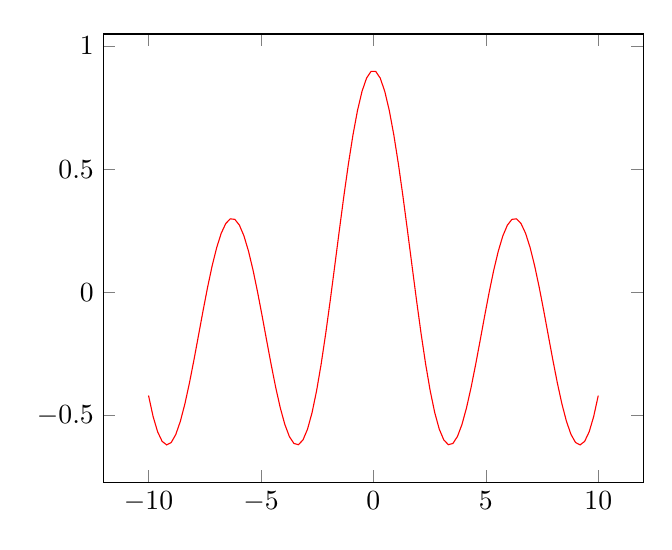
\begin{tikzpicture}
		\begin{axis}
			\addplot[
				color=red,
				domain=-10:10,
				samples=100
			]{0.3 * cos(deg(0.5 * x)) + 0.6 * cos(deg(x))};
		\end{axis}
	\end{tikzpicture}
	\caption{An arbitrary even function}
	\label{fig:odd-arb-func}
\end{figure}

\paragraph*{}
From the principal premise, it is inferred that it is possible to express an
even periodic signal such as the one given in figure \ref{fig:odd-arb-func} as
a sum of cosine waves:
\begin{align*}
	f(t) &= \sum^{\infty}_{n=0}a_n \cos(2 \pi \nu n t) \\
	&= a_0 + a_1 \cos(2 \pi \nu t) + a_2 \cos (4 \pi \nu t) + a_3 (6 \pi \nu t) + \dots
\end{align*}

\paragraph*{}
Now the question of what the individual values of $a_n$ are is posed.

\paragraph*{}
A formula for calculating the values of $a_n$ is presented, as well as a
derivation.

\paragraph*{}
First, let us multiply the left-hand and the right-hand side by $\cos(2 \pi \nu
m t)$, where $m \in \mathbb{R}^+$.
$$f(t) \cos(2 \pi \nu m t) = \sum^{\infty}_{n=0}a_n \cos(2 \pi \nu n t) \cos(2
\pi \nu m t)$$

\paragraph*{}
Then, integration is done on both sides of the equation.
\begin{equation*} 
	\begin{aligned}
		\int\limits_{T} f(t) \cos(2 \pi \nu m t) dt &= \int\limits_{T} \sum^{\infty}_{n=0}
		a_n \cos(2 \pi \nu n t) \cos(2 \pi \nu m t) dt \\
		&= \int\limits_T a_0 \cos (2 \pi \nu m t) + a_1 \cos (2 \pi \nu t) \cos (2 \pi
		\nu m t) + a_2 \cos (4 \pi \nu t) \cos (2 \pi \nu m t) + \dots dt \\
		&= \int\limits_T a_0 \cos (2 \pi \nu m t) dt + \int\limits_T a_1 \cos (2 \pi \nu t)
		\cos (2 \pi \nu m t) dt + \dots \\
	\end{aligned}
\end{equation*}

\paragraph*{}
Since the values of $a_n$ are constant real numbers, it follows that the
integral of the sum can be expressed as follows:
\begin{equation*}
	\begin{aligned}
		\int\limits_T f(t) \cos (2 \pi \nu m t) dt &= \sum^{\infty}_{n=0} \left( a_n
		\int\limits_{T} \cos(2 \pi \nu n t) \cos(2 \pi \nu m t) dt \right) \\
	\end{aligned}
\end{equation*}

\paragraph*{}
Let us now employ the trigonometric product identity:
\begin{equation}
	\int\limits_T \cos (2 \pi \nu n t) \cos (2 \pi \nu m t) dt = \frac{1}{2}
	\sum^{\infty}_{n=0} \left( a_n \int\limits_T  \cos \left( \left( m + n \right) 2
	\pi \nu t \right) + \cos \left( \left( m - n \right) 2 \pi \nu t \right) dt
	\right)
	\label{eqn:fourier-series-1}
\end{equation}

Since $m \geq 0$, and since $m$ is an integer (making $m + n$ an integer), it
follows that $\cos \big((m + n) 2 \pi \nu t \big)$ has $m + n$ oscillations in
a period. Since this is true, when this function is integrated, due to the
orthogonality of cosines:
$$\int\limits_T \cos \left( \left(m + n \right) 2 \pi \nu t \right) dt = 0$$

Equation \ref{eqn:fourier-series-1} is then simplified to:
\begin{equation}
	\int\limits_{T} f(t) \cos(2 \pi \nu m t) dt = \frac{1}{2} \sum^{\infty}_{n=0} a_n
	\int\limits_{T} \cos( (m - n) 2 \pi \nu t) dt
	\label{eqn:fourier-series-2}
\end{equation}

\paragraph*{}
Since the cosine function is even, in one period (ie. the interval of the
integration - from $-\frac{T}{2}$ to $\frac{T}{2}$) the following is true:
$$\cos( (m - n) 2 \pi \nu t) = \cos( (n - m) 2 \pi \nu t)$$

\paragraph*{}
When $m = n$:
$$\cos( (m - n) 2 \pi \nu t) = \cos(0) = 1$$

\paragraph*{}
To consider the case of $m - n$, we must acknowledge the fact that the cosine
function will complete $\left| m - n \right|$ oscillations in a single period.
Since the interval of integration is one period, it follows that:
$$\int\limits_T \cos( (m - n) 2 \pi \nu t) dt = \int\limits_T 1 \cdot dt$$

\paragraph*{}
Summing up:
\[
	\int\limits_{T} \cos( (m - n) 2 \pi \nu t) = 
	\begin{cases}
		\int\limits_{T} \cos ( (m -n) 2 \pi \nu t) dt = 0 & \text{when } m \neq n \\
		\int\limits_{T} 1 \cdot dt = T & \text{when } m = n
	\end{cases}
\]

\paragraph*{}
Let us observe the summation in equation \ref{eqn:fourier-series-2}. In the
summation, it can be observed that every term, except for the one where $m = n$
is equal to zero, and does not contribute to the series. Then, the summation
can be reduced exclusively to the case when $m=n$.
$$\int\limits_T f(t) \cos(m 2 \pi \nu t) dt = \frac{1}{2} a_m T$$
Then $a_m$ is:
\begin{equation*}
	a_m = \frac{2}{T} \int\limits_T f(t) \cos(m 2 \pi \nu t) dt
\end{equation*}
We can replace $m$ with $n$, since $m$ did not contribute to the original
equation:
\begin{equation}
	a_n = \frac{2}{T} \int\limits_T f(t) \cos(m 2 \pi \nu t) dt
	\label{eqn:fourier-series-amp}
\end{equation}

Substituting with $m = 0$ for $a_0$ in equation \ref{eqn:fourier-series-1}, we
get:
$$
\begin{aligned}
	\int\limits_{T} f(t) \cos(2 \pi \nu m t) dt &= \sum_{n=0}^{\infty} a_n \int\limits_T \cos
	( 2 \pi \nu n t) dt \\
	\int\limits_T f(t) dt &= T a_0
\end{aligned}$$
This gives the final result for the $y$ axis offset:
\begin{equation}
	a_0 = \frac{1}{T} \int\limits_T f(t) dt
	\label{eqn:fourier-series-yoffset}
\end{equation}

\paragraph*{}
For even functions, we have derived a formula for the amplitudes of the terms
in the series.

\paragraph*{}
Odd functions are represented with sine waves:
$$f_o(t) = \sum^{\infty}_{n=1} b_n \sin(2 \pi \nu n t)$$
It can similarly be shown that the amplitude of each constituting sine wave
$b_n$ is given by:
$$b_n = \frac{2}{T}\int\limits_T f_o(t) \sin(2 \pi \nu n t) dt$$
The derivation is similar to that of even functions and is therefore omitted.

\paragraph*{}
Finally, the individual even and odd constituents' formulae can be combined to
satisfy the requirement of the original premise that any waveform can be
represented as a sum of sine and cosine waves:
$$f(t) = a_0 + \sum^{\infty}_{n=1} (a_n \cos(2 \pi \nu n t) + b_n \sin(2 \pi
\nu n t))$$
where
\begin{align*}
	a_0 &= \frac{1}{T} \int\limits_T f(t) dt \\
	a_n &= \frac{2}{T} \int\limits_T f(t) \cos(2 \pi \nu n t) dt, n \neq 0 \\
	b_n &= \frac{2}{T} \int\limits_T f(t) \sin(2 \pi \nu n t) dt \\
\end{align*}

Euler's formulae allow for expressing the Fourier series in complex form:
$$cos \theta = \frac{e^{i\theta} + e^{-i\theta}}{2}$$
$$sin \theta = \frac{e^{i\theta} - e^{-i\theta}}{2i}$$
\begin{equation*}
	\begin{aligned}
		f(t) &= a_0 + \sum^{\infty}_{n=1}(a_n \cos(2 \pi \nu n t) + b_n \sin(2
		\pi n \nu t)) \\
		& = a_0 + \sum^{\infty}_{n=1}\Big(
		a_n \frac{e^{i 2 \pi \nu n t} + e^{-i 2 \pi \nu n t}}{2} + 
		b_n \frac{e^{i 2 \pi \nu n t} - e^{-i 2 \pi \nu n t}}{2i}\Big) \\
		&= a_0 + \sum^{\infty}_{n=1} \frac{a_n - ib_n}{2}e^{2 \pi \nu n t} +
		\sum^{\infty}_{n=1} \frac{a_n + ib_n}{2} e^{-2 \pi \nu n t}
	\end{aligned}
\end{equation*}

To solve the issue of having different complex exponentials let us set $n$ to
be $n = -n$ in the first summation:
\begin{equation}
f(t) = a_0 + \sum_{n=-1}^{-\infty} \frac{a_{-n} - i b_{-n}}{2} e^{- 2 \pi \nu n
t} + \sum_{n=1}^{\infty} \frac{a_n + i b_n}{2} e^{-2 \pi \nu n t}
\label{eqn:complex-fourier}
\end{equation}

Let us also define the following:
\begin{equation*}
	\begin{aligned}
		c_0 &= a_0 \\
		c_{n+} &= \frac{a_n + i b_n}{2} \\
		c_{n-} &= \frac{a_n - i b_n}{2} \\
	\end{aligned}
\end{equation*}

Then, with these defined, we can rewrite equation \ref{eqn:complex-fourier}
as\footnote{This is often referred to as the \textit{synthesis} equation.}:
\begin{equation}
	f(t) = \sum^{\infty}_{n = - \infty} c_n e^{-i 2 \pi \nu n t}
	\label{eqn:complex-fourier-series}
\end{equation}

\paragraph*{}
$c_n$ is expressed in the following\footnote{This equation is referred to as
the \textit{analysis} equation.}:
\begin{equation}
	\begin{aligned}
		c_n &= 
		\frac{1}{2} \cdot \bigg( \frac{2}{T} \int\limits_T f(t) \cos(2 \pi \nu n t) dt
		- i \frac{2}{T} \int\limits_T f(t) \sin(2 \pi \nu n t) dt \bigg) \\
		&= \frac{1}{T} \int\limits_T f(t) \cos(2 \pi n \nu t) - i f(t) \sin(2 \pi \nu
		n t) dt \\
		&= \frac{1}{T} \int\limits_T f(t) \bigg( \frac{e^{i 2 \pi \nu n t} + e^{-i 2
		\pi \nu n t}}{2} - i \frac{e^{i 2 \pi \nu n t} - e^{-i 2 \pi \nu n
		t}}{2i} \bigg) \\
		&= \frac{1}{T} \int\limits_T f(t) \frac{2 e^{i 2 \pi \nu n t}}{2} dt \\
		c_n &= \frac{1}{T} \int\limits_T f(t) e^{i 2 \pi \nu n t} dt
	\end{aligned}
	\label{eqn:fourier-analysis}
\end{equation}

\subsection{The Fourier transformation}

\paragraph*{}
The Fourier transformation, unlike the Fourier series which operates on
periodic functions, operates on non-periodic functions. This is achieved based
on the fact that a non-periodic function is expressible as a periodic function
whose interval is $\infty$.

\paragraph*{}
Its derivation is given in this subsection. Let us start from the Fourier
series.

\paragraph*{}
Next, let $\omega$ be:
$$\omega = 2 \pi \nu n$$

\paragraph*{}
This expression allows us to express equation \ref{eqn:fourier-analysis} as a
function of $\omega$:
\begin{equation}
	\begin{aligned}	
		\frac{1}{T} \int\limits_T f(t) e^{i 2 \pi \nu n t} dt &= \frac{1}{T} \int\limits_T
		f(t) e^{i \omega t} dt \\
		g(\omega) &= \frac{1}{T} \int\limits_T f(t) e^{i \omega t} dt \\
	\end{aligned}
\end{equation}

\paragraph*{}
Rewriting equation \ref{eqn:complex-fourier-series} we get:
$$f(t) = \sum_{n = - \infty}^{\infty} g(\omega) e^{-i \omega t}$$
Note that this equation connects the time and frequency domains.

\paragraph*{}
Substituting:
\begin{equation}
	\begin{aligned}
	f(t) &= \sum_{n = - \infty}^{\infty} \left( \frac{1}{T} \left(
	\int\limits_{-\frac{T}{2}}^{\frac{T}{2}} f(t) e^{i \omega t} dt\right)e^{-i \omega
	t} \right)
	\end{aligned}
	\label{eqn:substituted-cplx-f-series}
\end{equation}

\paragraph*{}
Let us now find the difference between the two terms $\Delta \omega$:
\begin{equation*}
	\begin{aligned}
		\Delta \omega &= \omega_{n+1} - \omega{n-1} \\
		&= ((n + 1)2 \pi \nu) - (n 2 \pi \nu) \\
		&= \pi \nu \\
		&= \frac{2 \pi}{T}
	\end{aligned}
\end{equation*}

\paragraph*{}
Let us solve equation \ref{eqn:substituted-cplx-f-series} for $T = \frac{2 \pi}
{\Delta \omega}$.
\begin{equation*}
	\begin{aligned}
		f(t) &= \sum_{n = - \infty}^{\infty} \left( \frac{\Delta
			\omega}{\pi} \left(
	\int\limits_{-\frac{T}{2}}^{\frac{T}{2}} f(t) e^{i \omega t} dt\right)e^{-i \omega
	t} \right)
	\end{aligned}
\end{equation*}

\paragraph*{}
Now, let $T$ approach $\infty$ as per the definition of the Fourier
transformation:
$$T \rightarrow \infty$$

Conversely:
$$\lim_{T \rightarrow \infty} \Delta \omega = 0$$

\paragraph*{}
Since $\Delta \omega \rightarrow 0$, the function becomes continuous. Because
of this, we can express the sum as a Riemann sum. Note that $\Delta \omega$
becomes $d \omega$:
\begin{equation}
	\begin{aligned}
		f(t) &= \sum_{n = - \infty}^{\infty} \left( \frac{\Delta \omega}{\pi}
		\left( \int\limits_{-\infty}^{\infty} f(t) e^{i \omega t}
		dt\right)e^{-i \omega t} \right) \\
		&= \int\limits_{- \infty}^{\infty} \left(
		\int\limits_{-\infty}^{\infty} f(t) e^{i \omega t} dt\right)e^{-i
		\omega t} \frac{d \omega}{\pi} \\
		&= \frac{1}{\pi} \int\limits_{- \infty}^{\infty} \left(
		\int\limits_{-\infty}^{\infty} f(t) e^{i \omega t} dt\right)e^{-i
		\omega t} d \omega
	\end{aligned}
	\label{eqn:riemann-fourier}
\end{equation}

\paragraph*{}
Trivially, it can be shown that equation \ref{eqn:riemann-fourier} is equal to:
$$f(t) = \frac{1}{\pi} \int\limits_{-\infty}^{\infty} g(\omega) e^{- i \omega t}
dt$$

\paragraph*{}
The operation $\hat{f}(t)$ is defined to be $g(\omega)$:
$$\hat{f}(t) = g(\omega) = \int\limits_{-\infty}^{\infty} f(t) e^{i \omega t}
dt$$

\paragraph*{}
This is the Fourier transformation.

\paragraph*{}
This equation gives a continuous relationship between frequency and amplitude,
which allows for identifying individual constituting waveforms inside complex
waveforms. Its applications are almost limitless - from analogue signal, to
digital signal processing, image processing, seismic analysis and even medicine.

\section{The chord identification algorithm}

\subsection{Definitions}

\paragraph*{}
A few more definitions are necessary for a clearer understanding of the
algorithm.

\paragraph*{}
A \textit{sample}, in this context, is a discrete measurement of a physical
waveform and its storage in a digital format. Usually, computers sample a
signal $44000$ times every second.

\paragraph*{}
The \textit{sampling frequency} $F_s$ of a digital audio recording is the
number of samples that is created by a digital recording device in a second.

\paragraph*{}
Let us define a convenience operation $\#(v)$ such that it returns the number
of dimensions of the vector space containing the vector $v$. To exemplify:
$$\# \left( \begin{bmatrix} a \\ b \\ c\end{bmatrix} \right) = 3$$

$$\# \left( \begin{bmatrix} a \\ b \\ c \\ d \end{bmatrix} \right) = 4$$
where $a$, $b$, $c$ and $d$ are real numbers.

\paragraph*{}
Let us define our final convenience operation $v = \text{append}(v, b)$ which
appends a value $b$ to a vector $v$. For example:
$$
v =
\begin{bmatrix}
	2 \\
	8 \\
	3 \\
\end{bmatrix}
$$
$$
\text{append}\left( v, 4 \right) =
\begin{bmatrix}
	2 \\
	8 \\
	3 \\
	4 \\
\end{bmatrix}
$$

\paragraph*{}
Let a \textit{symmetric vector} be such a vector:
$$a =
\begin{bmatrix}
	a_0 \\
	a_1 \\
	\vdots \\
	a_{\left( \frac{n}{2} - 1 \right)} \\
	a_{\frac{n}{2}} \\
	a_{\left( \frac{n}{2} + 1 \right) } \\
	\vdots \\
	a_{n-1} \\
	a_n
\end{bmatrix}
$$
with the following set of properties:
$$
\left\{
	 a_{\left( \frac{n}{2} - 1 \right)} = a_{\left( \frac{n}{2} + 1 \right)}
	 \dots a_1 = a_{n-1}, a_0 = a_n , n = 2l + 1 : l \in \mathbb{Z}^+
\right\}
$$

\paragraph*{}
Let us define another convenience function $\text{max}(v)$, which for a vector
$v$ returns the numerically largest dimension. For example:
$$
\text{max} \left(
	\begin{bmatrix}
		5 \\
		9 \\
		2 \\
	\end{bmatrix}
\right) = 9
$$

\paragraph*{}
A \textit{Discrete Fourier transformation} can be thought of as a discrete
counterpart to the continuous Fourier transformation previously discussed.
Unlike the Fourier series, it can operate on non-periodic signals, and for a
sufficiently small value of $\Delta \omega$ the error produced is negligible.
Let it be denoted as:
$$a = \text{dft}(b, c)\text{ where $b$ is the domain of the waveform and $c$ is
the codomain}$$
Such a function returns values of the amplitudes of the constituting waveforms
and stores them in a vector here denoted as $a$.

\subsection{The algorithm}

\paragraph*{} 
Given an input signal such as the one given in figure \ref{fig:input-signal}, 
the algorithm operates in $4$ distinct stages.
\begin{figure}
	\centering
	\begin{tikzpicture}[scale=1.1]
		\begin{axis}[enlargelimits=false,axis on top,xlabel = Time
					   (\si{s}), ylabel = Amplitude]
		   \addplot graphics
		   [xmin=0,xmax=20,ymin=15000,ymax=22000]
		   {img/input-signal};
		\end{axis}
	\end{tikzpicture}
	\caption{An example of an input signal - in this case a $C_{maj}$ chord}
	\label{fig:input-signal}
\end{figure}

\paragraph*{}
The computer is initially instructed to count the number of samples $n$ in the
digital recording.

\paragraph*{}
The computer is instructed to load the samples of the signal in a column vector
$A$.
$$A =
\begin{bmatrix}
	a_1 \\
	a_2 \\
	a_3 \\
	\vdots \\
	a_{n}
\end{bmatrix}\text{where $a$ is the sample value and $n$ is the number of
samples}
$$
Note that these are the values represented on the $y$ axis in figure
\ref{fig:input-signal}.

\paragraph*{}
To get the values of the $x$ axis, ie. the time domain, it is necessary to
create a column vector as such.
$$t = \frac{1}{F_s} \cdot
\begin{bmatrix}
	0 \\
	1 \\
	2 \\
	\vdots \\
	n-1 \\
\end{bmatrix}
$$
These two vectors possess the property $\#(A) = \#(t)$.

\paragraph*{}
With these values, it is possible to proceed in the algorithm.

\subsection{The Fourier transformation}
A discrete Fourier transformation is done on the vectors
$$F = \text{dft}(t, A)$$
The Fourier transformation, for real inputs, gives a symmetric vector $F$. Due
to the unnecessary values in $F$ it is cut off at the middle part onwards.
$$F' =
\begin{bmatrix}
	F_1 \\
	F_2 \\
	F_3 \\
	\vdots \\
	F_{\frac{\#(F) - 1}{2}}
\end{bmatrix}
$$
Since the numbers given by the Fourier transformation are complex, to get the 
amplitudes of the frequencies it is necessary to get absolute values for all 
of the values in the vector given by the Fourier transformation.
$$F'' = 
\begin{bmatrix}
	|F'_1| \\
	|F'_2| \\
	|F'_3| \\
	\vdots \\
	\left| F'_{\#(F')} \right|
\end{bmatrix} =
\begin{bmatrix}
	\sqrt{\Re(F'_1)^2 + \Im(F'_1)^2} \\
	\sqrt{\Re(F'_2)^2 + \Im(F'_2)^2} \\
	\sqrt{\Re(F'_3)^2 + \Im(F'_3)^2} \\
	\vdots \\
	\sqrt{\Re \left( F'_{\#(F')} \right) ^2 + \Im \left( F'_{\#(F')} \right)^2}
\end{bmatrix}
$$

\paragraph*{}
A vector $f$ is created to store the domain of the Fourier transformation, 
such that it is a linear space from $0$ to $1$ with the norm being equal to 
the one returned Fourier transformation, multiplied by the sampling frequency 
of the original file. This is in turn, creates the frequency domain.
$$f = F_s \cdot
\begin{bmatrix}
	0 \\
	1 \cdot \frac{1}{\#(F'')} \\
	2 \cdot \frac{1}{\#(F'')} \\
	\vdots \\
	\left( \#(F'') - 1 \right) \cdot \frac{1}{\#(F'')} \\
	\#(F'') \cdot \frac{1}{\#(F'')} \\
\end{bmatrix}
$$

\subsection{Fourier transform peak identification} 
\paragraph*{}
In this section of the algorithm the computer tries to identify which peaks 
play a significant role in composing a chord. 

\paragraph*{} 
Due to the possibility of different waveforms having different amplitudes, and
therefore the possibility of their respective Fourier transformations having
different amplitudes, it is impossible to compare them before normalizing them.
To normalize them (ie. make their maximal values the same) the existing vector
is multiplied by the reciprocal of the largest dimension in it:
$$F''' = \frac{1}{\text{max(}F''\text{)}} \cdot F''$$

\paragraph*{}
It can be assumed that there are insignificant frequencies that do not play a
role in a chord, but may be present (noise, instrument insignificant noises,
like the moving of the piston on a trumpet, or the actual picking of the
string). So, to improve the algorithm, it was decided to take values which are
numerically larger than a certain constant value, named cutoff value and
denoted as $c_o$. This was achieved using the following logical condition. 
$$p = \varnothing$$
$$\forall v \in F''' : \bigg(v > c_o \Rightarrow p = \text{append}\left(p, v
\right) \bigg)$$
As an example, the normalized Fourier transformation, alongside the cutoff 
value of $c_o = 0.15$, is plotted in figure \ref{fig:fourier-signal}.
\begin{figure}[ht]
	\centering
	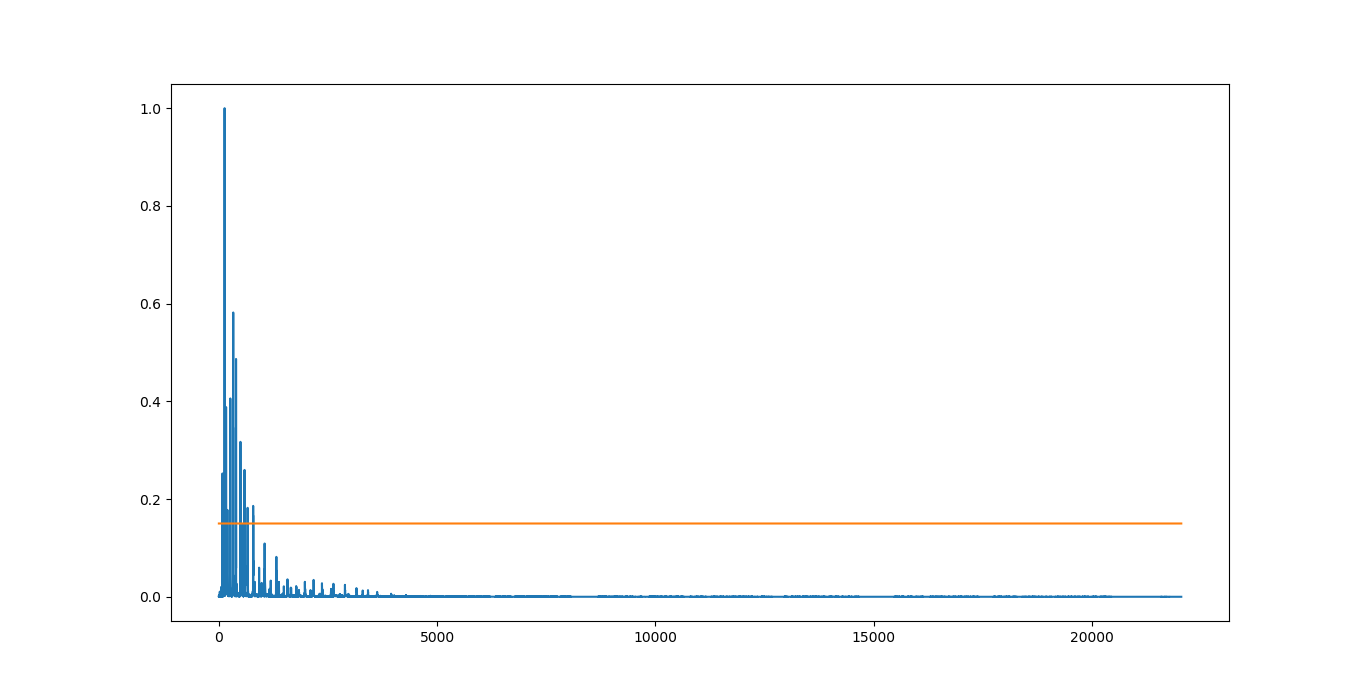
\includegraphics[width=\textwidth]{img/fourier-signal}
	\caption{The normalized Fourier transformation of the signal given in 
	figure \ref{fig:input-signal}, ie. a $C_{maj}$ chord.}
	\label{fig:fourier-signal}
\end{figure}

\paragraph*{} 
Due to the fact that the Fourier transform is continuous, the apparent peaks of
the Fourier transform are not discrete values, but are rather reminiscent of
the peaks shown in figure \ref{fig:conc-triang}.
\begin{figure}[ht]
	\centering
	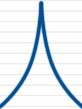
\includegraphics[width=0.1 \textwidth]{img/conv-triangle}
	\caption{An example of how the peaks are (\textit{Is There A One-Line
		Function That Generates A Triangle Wave?})}
	\label{fig:conc-triang}
\end{figure}

To resolve this issue, the average of neighboring values of a peak is
calculated.  Neighboring values $w$ are defined to be neighboring to a value
$v$ if the absolute difference between them is less than a leeway value $l$.
$$p' = \varnothing$$
$$\forall v \in p : \left( 
	\left( \left( w \not\in p' : \abs{v - w} < l \right) \rightarrow p' =
		\text{append}\left( p', w \right) 
	\right) \land
	\left( \left( w \in p' : \abs{v - w} < l \right) \rightarrow
	w = \frac{(w + v)}{2}
	\right)
\right)$$
At this point, the vector $p'$ contains the frequencies of the played chord 
that are more intense than a given cutoff value.

\subsection{Note identification}
Notes are identified in this step by finding the closest value in a look-up 
table of frequencies\footnote{This table is available at the following link: 
\url{https://pages.mtu.edu/~suits/notefreqs.html}.}. In this subsection the
methodology for finding the note is presented. In this section, let us denote
any value in $p'$ as $v$. Let us also denote the lookup table as a column
vector $r$. We start from the premise that $v$ lies between two closest values
in $r$:
$$r_n \leq v \leq r_{n+1}$$
The closest value is evaluated to be the expected note:
$$\left( | v - r_n | > | v - r_{n+1} | \Rightarrow e = r_{n+1} \right) \land
\left( | v - r_n | < | v - r_{n+1} | \Rightarrow e = r_{n} \right)$$
where $e$ is the final note.

\subsection*{}
\paragraph*{}
The full algorithm is available at the following link:
\url{https://github.com/markovejnovic/Chordy}.

\subsection{Chord identification}
\paragraph*{}
Since this algorithm is only designed for chord triads, it was not difficult 
to design an algorithm which identifies chords from the previously identified 
notes. A simple look-up table was created and a simple searching algorithm was 
implemented.

\section{Evaluation}

\paragraph*{}
This paper defines an arbitrary success rate as the ration between the number
correctly analyzed chords (as per the chord played on an instrument) and the
number of chords analyzed in total.

\paragraph*{}
To identify how well the algorithm performs tests were created. $10$ guitar 
chord samples were downloaded from the internet (\textit{vide} the works 
cited). These chord samples were then analyzed using the algorithm. Since it 
was known which chords were played, it was possible to determine the success
rate of the algorithm.

\paragraph*{}
For a value of $c_o = 0.15$, the algorithm's success rate was $60\%$. However, 
when the value of $c_o$ was chosen to be a value greater or lesser than $0.15$ 
different success rates were achieved. A plot of the relationship between 
$c_o$ and the success rate of the algorithm is given in figure 
\ref{fig:success-rate}.
\begin{figure}[ht]
	\centering
	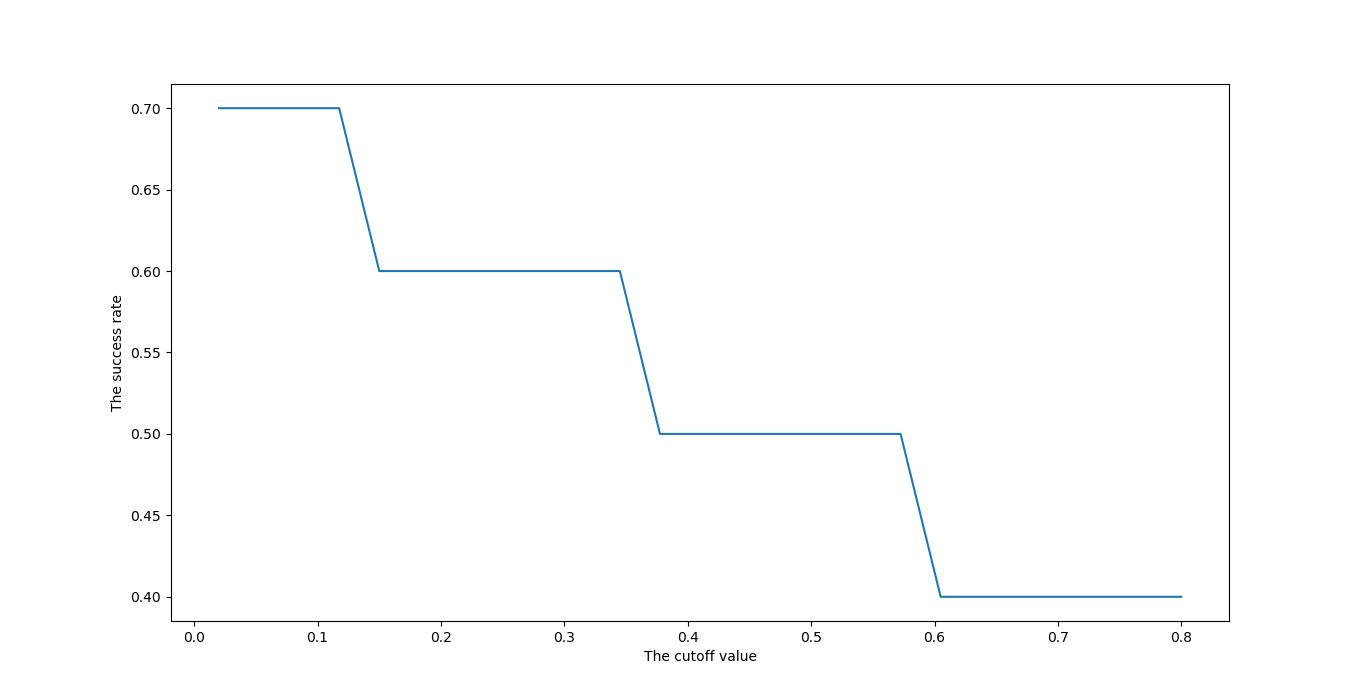
\includegraphics[width=\textwidth]{img/success-rate}
	\caption{The relationship between $c_o$ and the success rate of the 
	algorithm.}
	\label{fig:success-rate}
\end{figure}

\paragraph*{}
It is obvious that the maximal success rate is achieved for the minimal value 
of $c_o = 0.02$. This success rate is equal to $70\%$. Note, however, that 
the chords played in the samples might have not been the ones that the authors 
stated they were. It is possible that the guitars the chords were played on 
were out of tune, or the chords were played improperly, or the tune of the 
guitars was not one of $A_4 = 440$, or it is even possible that the guitars 
used were not precisely manufactured.

\paragraph*{}
Figure \ref{fig:success-rate} also contains a negative linear fit which
predicts that at $c_o = 0$ the success rate is $0.7086$, ie. $70.9\%$.

\section{Conclusion}
\paragraph*{}
The algorithm seems effective in achieving the required result. The evaluation 
of the algorithm was incomplete, due to a lack of chord samples. For more 
accurate evaluation it is necessary to use better chord samples.

\paragraph*{}
With a success rate higher than $70\%$, this algorithm can be used for roughly
estimating chords, but cannot be used for rigorous musical analysis.

\clearpage
\pagebreak
\pagenumbering{gobble}
\section*{Works cited}
\begin{hangparas}{.25in}{1}

\begin{sloppypar}
	``A Minor Chord (Ringout)''. Freesound.Org, 2014,
	\url{https://freesound.org/people/dxe10/sounds/234061/}. Accessed 6 Oct
	2018.\\	
\end{sloppypar}

Benward, Bruce, and Marilyn Nadine Saker. 
\textit{Music In Theory And Practice}. Mcgraw-Hill, 2009. \\

``Frequencies Of Musical Notes, A4 = 440 Hz''. \textit{Pages.Mtu.Edu}, 2018, 
\url{https://pages.mtu.edu/~suits/notefreqs.html}. Accessed 3 Aug 2018. \\

``Guitar - Major Chords Pack''. Freesound.Org, 2018, 
\url{https://freesound.org/people/danglada/packs/1011/}. Accessed 6 Oct 2018. \\

Hausner, Christoph. \textit{``Design And Evaluation Of A Simple Chord 
Detection Algorithm''}. University Of Passau, 2014. \\

\begin{sloppypar}
	``Integral Over A Period Interval''. \textit{Planetmath.Org}, 2018,
	\url{http://planetmath.org/integraloveraperiodinterval}. Accessed 31 July
	2018.  \\
\end{sloppypar}

\textit{Is There A One-Line Function That Generates A Triangle Wave?}. 2009,
\url{https://stackoverflow.com/questions/1073606/is-there-a-one-line-function-that-generates-a-triangle-wave}.
Accessed 5 Dec 2018.

Muludi, Kurnia, Aristoteles, and Abe Frank SFB Loupatty. \textit{``Chord 
Identification Using Pitch Class Profile Method With Fast Fourier Transform 
Feature Extraction''}. International Journal Of Computer Science Issues, vol 
11, no. 3, 2018, pp. 139-144. \\

Shazam Entertainment, Ltd. \textit{An Industrial-Strength Audio Search 
Algorithm}. 2018, 
\url{http://www.ee.columbia.edu/~dpwe/papers/Wang03-shazam.pdf}. 
Accessed 30 July 2018. \\

Smith III, Julius. ``Positive And Negative Frequencies.
\textit{Ccrma.Stanford.Edu}, 2018,
\url{https://ccrma.stanford.edu/~jos/mdft/Positive_Negative_Frequencies.html}.
Accessed 3 Dec 2018. \\

Valente, Michael et al. \textit{Audiology}. Thieme, 2008. \\

Weisstein, Eric W. ``Orthogonal Functions''. \textit{Mathworld.Wolfram.Com},
\url{http://mathworld.wolfram.com/OrthogonalFunctions.html}. Accessed 29 Nov 2018. \\

\end{hangparas}
\end{document}
